%!TEX TS-program = xelatex
\documentclass[a4paper,14pt]{article}
\usepackage[utf8]{inputenc}
\usepackage[T1]{fontenc}

%%% Работа с русским языком
\usepackage[english,russian]{babel}   %% загружает пакет многоязыковой вёрстки

%\usepackage{polyglossia}    %для русского языка
%\usepackage{xecyr}          %кириллические символы
%\setdefaultlanguage{russian}  %% устанавливает главный язык документа
%\setotherlanguage{english} %% объявляет второй язык документа

\usepackage{fontspec}      %% подготавливает загрузку шрифтов Open Type, True Type и др.
\defaultfontfeatures{Ligatures={TeX},Renderer=Basic}  %% свойства шрифтов по умолчанию
\setmainfont[Ligatures={TeX,Historic}]{Times New Roman} %% задаёт основной шрифт документа
\setsansfont{Comic Sans MS}                    %% задаёт шрифт без засечек
\setmonofont{Courier New}
\usepackage{indentfirst}
\frenchspacing

\renewcommand{\epsilon}{\ensuremath{\varepsilon}}
\renewcommand{\phi}{\ensuremath{\varphi}}
\renewcommand{\kappa}{\ensuremath{\varkappa}}
\renewcommand{\le}{\ensuremath{\leqslant}}
\renewcommand{\leq}{\ensuremath{\leqslant}}
\renewcommand{\ge}{\ensuremath{\geqslant}}
\renewcommand{\geq}{\ensuremath{\geqslant}}
\renewcommand{\emptyset}{\varnothing}

%%% Дополнительная работа с математикой
\usepackage{amsmath,amsfonts,amssymb,amsthm,mathtools} % AMS
\usepackage{icomma} % "Умная" запятая: $0,2$ --- число, $0, 2$ --- перечисление

%% Номера формул
%\mathtoolsset{showonlyrefs=true} % Показывать номера только у тех формул, на которые есть \eqref{} в тексте.
%\usepackage{leqno} % Нумерация формул слева	

%% Перенос знаков в формулах (по Львовскому)
\newcommand*{\hm}[1]{#1\nobreak\discretionary{}
{\hbox{$\mathsurround=0pt #1$}}{}}

%%% Работа с картинками
\usepackage{graphicx}  % Для вставки рисунков
\graphicspath{{images/}}  % папки с картинками
\setlength\fboxsep{3pt} % Отступ рамки \fbox{} от рисунка
\setlength\fboxrule{1pt} % Толщина линий рамки \fbox{}
\usepackage{wrapfig} % Обтекание рисунков текстом

%%% Работа с таблицами
\usepackage{array,tabularx,tabulary,booktabs} % Дополнительная работа с таблицами
\usepackage{longtable}  % Длинные таблицы
\usepackage{multirow} % Слияние строк в таблице
\usepackage{float}% http://ctan.org/pkg/float

%%% Программирование
\usepackage{etoolbox} % логические операторы


%%% Страница
\usepackage{extsizes} % Возможность сделать 14-й шрифт
\usepackage{geometry} % Простой способ задавать поля
\geometry{top=20mm}
\geometry{bottom=20mm}
\geometry{left=20mm}
\geometry{right=10mm}
%
%\usepackage{fancyhdr} % Колонтитулы
% 	\pagestyle{fancy}
%\renewcommand{\headrulewidth}{0pt}  % Толщина линейки, отчеркивающей верхний колонтитул
% 	\lfoot{Нижний левый}
% 	\rfoot{Нижний правый}
% 	\rhead{Верхний правый}
% 	\chead{Верхний в центре}
% 	\lhead{Верхний левый}
%	\cfoot{Нижний в центре} % По умолчанию здесь номер страницы

\usepackage{setspace} % Интерлиньяж
\onehalfspacing % Интерлиньяж 1.5
%\doublespacing % Интерлиньяж 2
%\singlespacing % Интерлиньяж 1

\usepackage{lastpage} % Узнать, сколько всего страниц в документе.

\usepackage{soul} % Модификаторы начертания

\usepackage[hyphens]{url}
\usepackage{hyperref}
\usepackage[usenames,dvipsnames,svgnames,table,rgb]{xcolor}
\hypersetup{                % Гиперссылки
    unicode=true,           % русские буквы в раздела PDF
    pdftitle={},   % Заголовок
    pdfauthor={},      % Автор
    pdfsubject={},      % Тема
    pdfcreator={}, % Создатель
    pdfproducer={}, % Производитель
%    pdfkeywords={keyword1} {key2} {key3}, % Ключевые слова
    colorlinks=true,        % false: ссылки в рамках; true: цветные ссылки
    linkcolor=black,          % внутренние ссылки
    citecolor=black,        % на библиографию
    filecolor=magenta,      % на файлы
    urlcolor=black           % на URL
}
\makeatletter
\def\@biblabel#1{#1. }
\makeatother
\usepackage{cite} % Работа с библиографией
%\usepackage[superscript]{cite} % Ссылки в верхних индексах
%\usepackage[nocompress]{cite} % 
\usepackage{csquotes} % Еще инструменты для ссылок

\usepackage{multicol} % Несколько колонок

\usepackage{tikz} % Работа с графикой
\usepackage{pgfplots}
\usepackage{pgfplotstable}

\usepackage{ dsfont }

\newcommand{\imref}[1]{рис.~\ref{#1}}

\usepackage{multirow}
\usepackage{spreadtab}
\newcolumntype{K}[1]{@{}>{\centering\arraybackslash}p{#1cm}@{}}


\usepackage{xparse}
\usepackage{fancyvrb}

\RecustomVerbatimCommand{\VerbatimInput}{VerbatimInput}
{
    fontsize=\footnotesize
}

\newcolumntype{?}[1]{!{\vrule width #1}}

\usepackage{tocloft}
\renewcommand{\cftsecleader}{\cftdotfill{\cftdotsep}}

\usepackage{pdfpages}

\usepackage{rotating}

\usepackage{pdflscape}

\usepackage{ragged2e}
\usepackage{microtype}

\usepackage{subcaption}

% Выравнивание по ширине без переносов слов
\justifying
\sloppy
\tolerance=500
\hyphenpenalty=10000
\emergencystretch=3em

% Подогнать таблицу под ширину страницы
\usepackage{adjustbox}

\usepackage{titlesec}

% ГОСТ заголовки таблицы
\usepackage[font=small]{caption}
\usepackage{makecell}

\renewcommand\thefigure{\arabic{section}.\arabic{figure}}
\DeclareCaptionLabelSeparator{deffis}{ -- } 
\captionsetup[figure]{justification=centering,labelsep=period} % Картинки по центру, с точкой после рис


\DeclareCaptionLabelFormat{rightline}{\rightline{\bothIfFirst{#1}{ }#2}}
%\captionsetup[table]{justification=centering,labelformat=rightline,labelsep=newline}
\captionsetup[table]{justification=raggedleft,labelformat=rightline,labelsep=newline}

\newcommand{\tablecaption}[1]{\addtocounter{table}{1}\small \begin{flushright}
                                                                \tablename \ \thetable
\end{flushright}%
    \begin{center}
        #1
    \end{center}}

\usepackage{enumerate}
\usepackage{lastpage}




%сноска с новым номером на кждоый странице
\usepackage[perpage]{footmisc}
 
\DeclareCaptionLabelSeparator{deffis}{ -- } %разделитель объекта и названия






\usepackage[fixlanguage]{babelbib}
\usepackage{lastpage}
\begin{document}

    \begin{titlepage}
%    \begin{center}
%        ПРАВИТЕЛЬСТВО РОССИЙСКОЙ ФЕДЕРАЦИИ \\
%        ФЕДЕРАЛЬНОЕ ГОСУДАРСТВЕННОЕ АВТОНОМНОЕ \\
%        ОБРАЗОВАТЕЛЬНОЕ УЧРЕЖДЕНИЕ ВЫСШЕГО ОБРАЗОВАНИЯ\\
%        «НАЦИОНАЛЬНЫЙ ИССЛЕДОВАТЕЛЬСКИЙ УНИВЕРСИТЕТ\\
%        «ВЫСШАЯ ШКОЛА ЭКОНОМИКИ»
%    \end{center}

    \begin{center}
        \textbf{Федеральное государственное автономное образовательное
        	учреждение высшего образования 
        	«Национальный исследовательский университет 
        	«Высшая школа экономики».
        }
    
	\end{center}

%\vspace{6ex}
\vfill
	
	\begin{center}

        ОТЧЕТ \\
        	О НАУЧНО-ИССЛЕДОВАТЕЛЬСКОЙ РАБОТЕ \\
        	НА ТЕМУ:\\
        	<<Characterizing Graph Datasets for Node Classification:
        	Beyond Homophily–Heterophily Dichotomy>>
        

%        \vspace{2ex}

    \end{center}

    \vfill


    \begin{flushright}
        \textbf{Выполнили:}

        \vspace{2ex}

        Студенты группы мФТиАД21

        \vspace{2ex}
        
    \end{flushright}

    \vspace{5ex}
    \begin{center}
        Москва \the\year \, г.
    \end{center}

\end{titlepage}
\addtocounter{page}{1}
    
    \section*{\hfill РЕФЕРАТ \hfill}
    
    Расчетно-пояснительная записка \pageref{LastPage} с., 00 рис., 00 табл., 00 источников, 00 прил.
    
    КЛЮЧЕВЫЕ СЛОВА: ГРАФ, ГОМОФИЛИЯ, ГЕТОРОФИЛИЯ, GNN, КЛАССИФИКАЦИЯ, МЕТРИКА КАЧЕСТВА КЛАССИФИКАЦИИ, МЕТРИКА ГОМОФИЛИИ 
    
    \textbf{Объектом исследования в  НИР} являются метрики оценки гомофилии и качества классификации для графовых нейронных сетей для графов, подходящие для датасетов с различными размерами и количеством классов.
    
    \textbf{Целью НИРС} является формализация подходящих метрик качества классификации и гомофилии, теоретическое и эмпирическое доказательство их корректности, а также сравнение разных метрик между собой и выявление лучшей. 
    
    %Для выполнения НИРС использовались следующие \textbf{методы}:
    
    В результате выполнения НИРС были получены следующие \textbf{результаты}:
    
    \begin{itemize}
    	\item Получена метрика Adjusted Homophily, обладающая лучшими свойствами, по сравнению с существующими классическими метриками гомофилии. 
    
    	\item Получена метрика Label Informativeness (LI), подходящая для сравнения различных датасетов 
    
    	\item В результате серии экспериментов получено, что  для  GNN метрика Label Informativeness лучше, чем гомофилия.
    	Также получено, что LI объясняет, почему GNN иногда могут хорошо работать с гетерофильными наборами данных.
\end{itemize}

  
    \newpage
    
    \tableofcontents
    \pagebreak
    
    \newpage
    
	\section*{ \hfill ОБОЗНАЧЕНИЯ И СОКРАЩЕНИЯ \hfill}
	
	В работе  использованы следующие обозначения и сокращения:
	
	GNN	–	graph neural networks
	
	$LI$	–	Label Informativeness
	
	$E$	–	Ребра графа
	
	$V$	–	Вершины графа
	
	$G$	–	Граф
	
	$N(v)$	–	Соседи вершины $v$
	
	$d(V)$	–	Степень вершины $v$
	
	$X_v$	–	Вектор признаков
	
	$Y_v$	–	Метка класса 
	
	$p(.)$	–	Распределение меток класса
	
	\newpage
	
	\section*{ \hfill ВВЕДЕНИЕ \hfill}
	\addcontentsline{toc}{section}{\protect\numberline{}ВВЕДЕНИЕ}
	
	\textbf{Актуальность темы работы} обусловлена тем, что стандартные графовые нейронные сети плохо работают на негомофильных графах, однако, всё-таки могут достигать высокой производительности на некоторых графах с таким свойством.
	Поэтому важно иметь метрику, позволяющую отличать гомофильные и негомофильные случаи, так как для них требуются разные методы обучения.
	Также важно иметь метрику качества, показывающую стабильный результат на разных датасетах в разных задачах, чтобы сделать результаты интерпретируемыми и сопоставимыми. 
	
	\textbf{Целью работы} является определение метрики гомофолии графа, не зависящей от датасета и универсальной метрики качества GNN. 
	
	Для достижения поставленной цели в работе решаются следующие \textbf{основные задачи}:
	
	\begin{itemize}
		
	\item Исследование существующих метрик гомофилии и их недостатков
	
	\item Определение новой метрики гомофилии, которая закрывает недостатки классических метрик, и её теоретическое обоснование
	
	\item Определение новой метрики качества GNN, выходящей за пределы подхода гомофилии графов, и её теоретическое обоснование
	
	\item Эмпирическое сравнение полученных метрик
	
	\end{itemize}
	
	Решение поставленных задач осуществляется с использованием следующих \textbf{методов и подходов}: для определения метрик исследованы существующие подходы оценки гомофилии:
	
	\begin{enumerate}
		\item Гомофилия рёбер
		
		\item Гомофилия вершин
		
		\item Гомофилия классов
	\end{enumerate}

	А также определены необходимые свойства: 
	
	\begin{enumerate}
		\item Maximal agreement
		
		\item Minimal agreement
		
		\item Constant baseline
		
		\item Empty class tolerance
	\end{enumerate}
	
	И введены основные понятия:
	
	\begin{enumerate}
		\item Монотонность
		
		\item Модель конфигурации
		
		\item Асимптотическое константное предсказание
	\end{enumerate}
	
	При выполнении работы использованы следующие исходные данные:
	
	\begin{enumerate}
		\item Синтетические данные, полученные с помощью stochastic block model.
		
		\item Полусинтетические данные, полученные путем добавления ребер между классами разными способами к нескольким реальным графам, что даёт несколько наборов графов с разным уровнем гомофилии.
	
		\item Синтетические данные, сгенерированные согласно подходу, описанному в \cite{luan2021heterophily}.
	\end{enumerate}
	
	\pagebreak
    \section{Обзор литературы и направлений исследователей}
    \setcounter{figure}{0}
    
    \subsection{Обозначения}
    
    Возьмем простой ненаправленный граф $G = (V,E)$ с вершинами $V$, ребрами $E$.
    В каждой вершине $v$ есть вектор признаков $x_v$ и метка класса $y_v$.
    Пусть $n_k$ обозначает размер класса $k$. $N(v)$ – соседи вершины $v$ в $G$, $d(v)$ – степень вершины $v$.
    За $p(.)$ примем эмпирическое распределение меток класса.
    
    \subsection{Классические меры гомофилии}
    
    Свойство гомофилии определяет то, насколько похожие вершины графа связаны. Сходство оценивается в терминах меток вершин или  их признаков.
    
    Классическими мерами гомофилии являются:

	\begin{enumerate}
		\item Гомофилия рёбер определяется как доля ребер, связывающих вершины одного класса, в общем количестве ребер 
		$$h_{edge} = \dfrac{|\{\{u,v\} \in E : y_u = y_v\}|}{|E|}$$
		
		\item Гомофилия вершин определяется как усредненная по всем вершинам доля соседей, принадлежащих одному классу, в общем количестве вершин
		$$h_{node} = \dfrac{1}{n}\sum_{v \in V}\dfrac{|\{u \in N : y_u = y_v\}|}{d(v)}$$
		
		\item Гомофилия классов измеряется как отношение гомофилии текущей модели к гомофилии нулевой модели, где ребра не зависят от меток
		$$h_{class} = \dfrac{1}{C-1}\sum_{k=1}^{C}\left[ \dfrac{\sum_{v:y_v=k}|\{u \in N(v): y_u = y_v\}|}{\sum_{v:y_v=k}d(v)} - \dfrac{n_k}{n}\right]_+$$
	\end{enumerate}
	
	Меры 1 и 2 имеют существенный недостаток – они чувствительны к балансу классов и их количеству.
	Этих недостатков нет в гомофилия классов, однако, она не учитывает изменения степеней вершин и негомофильные классы. 
	
	\subsection{Критерии для меры гомофилии}
	
	В статье авторы опирались на работу Алексея Тинхонова и Людмилы Прохоренковой - Systematic analysis of cluster similarity indices: How to validate validation measures.
	В ней описаны критерии для метрик похожести кластеров, однако не все критерии метрик применимы для меры гомофилии.
	Например, критерий симметричности не применим для гомофилии, так как сравниваются разные сущности объектов - граф и класс объекта.
	Были взяты 4 критерия, которые подходят для меры гомофилии:
	
	\begin{itemize}
		\item Maximal agreement
		
		\item Minimal agreement
		
		\item Constant baseline
		
		\item Empty class tolerance baseline
	\end{itemize}
	
	\textbf{Maximal agreement}
	
	Это ограничение требуется, чтобы ввести максимальное значение метрики для графа, у которого все ребра соединяют только вершины своего класса (максимальная мера гомофильности).
	
	\textbf{Minimal Agreement} 
	
	Аналогично maximal agreement - для графа, у которого все ребра соединяют вершины разных классов (минимальная мера гомофиьльности).
	Максимальное и минимальное ограничение может казаться несущественным критериями, но важно, чтобы мера вела себя предсказуемо, что делает ее интерпретируемой.
	
	\textbf{Constant baseline}
	
	Это требование как раз решает недостатки гомофилии ребер и гомофилии вершин.
	Мера не должна зависеть от количества и распределений классов.
	Ожидается, что хорошая мера не должна отличаться в зависимости от количества классов.
	Также при случайной генерации сэмплов мера не должна давать различные результаты, то есть не сильно чувствительна к распределению внутри классов
	
	\textbf{Empty class tolerance baseline}
	
	Уточнение предыдущего ограничения: хорошая мера должна позволить сравнивать различные графы, но в графах может быть различное количество классов. Стандартное решение - добавить пустой класс, чтобы уравнять количество, при этом метрика должна быть нечувствительна к добавлению пустых классов.
	
	
	\subsection{Описание свойства Монотонности}
	
	Основываясь на работе “Good Classification Measures and How to Find Them”, авторы статьи заявляют о сопоставимости edge-wise метрик гомофилии и метрик качества классификации.
	Данное сравнение позволяет им развить метрику гомофилии по аналогии с классификационными метриками. Авторы приводят следующие рассуждения:
	
	При условии, что у ненаправленного графа каждое ребро ${u, v}$ дает две упорядоченные пары узлов $(u, v)$ и $(v, u)$, мы можем допустить, что для всех таких пар $(u, v)$ существуют лэйбл правдивых значений $y_u$ и лэйбл предсказаний $y_v$.
	При этом авторы замечают, что метрики классификации будут отражать соотношения этих двух лэйблов, а $edge-wise$ метрики в свою очередь демонстрируют как часто узлы, связанные ребром, принадлежат одному и тому же лэйблу.
	Из этого наблюдения авторы статьи выводят матрицу ошибок С с элементами $c_{ij}$, обозначающих количество ребер так, что $y_u = i$ и $y_v = j$, при этом отмечают, что такая матрица будет симметричной, так как граф не является направленным.
	
	Кроме того, отталкиваясь от заданной матрицы ошибок, авторы вводят новое определение монотонности метрики гомофилии, позволяющее сравнивать графы с различным количеством ребер и классов.
	Согласно этому определению, монотонной метрику можно считать при условии, что выполнена empty class tolerant, метрика возрастает при увеличении диагонального элемента на 2 и снижается при росте $с_{i,j}$ и $c_{j,i}$  на 1 для $i!=j$.
	
	Тем не менее, вернемся к рассмотрению эволюции метрики по аналогии с задачами классификации.
	Авторы, описывая усложнение показателей, приводят пары парамаетров точность - гомофилия ребер, сбалансированная точность - сбалансированная гомофилия.
	Переход от одной пары к другой подвержен одной логике -подобно тому, как точность может демонстрировать некорректные для принятия решений результаты на несбалансированной по классам выборке, гомофилия ребер ($h_{edge}$) также приводит к ошибочным выводам на таких выборках.
	С целью нивелировать данный эффект вводится мера сбалансированной гомофилии:
	
	$$h_{bal} = \dfrac{1}{C}\sum_{k=1}^{C}\dfrac{|(u,v) : y_u = y_v = k|}{D_k}$$
	
	Однако для такой метрики не выполняются критерии монотонности и asymptotic constant baseline.
	Для решения второй проблемы можно получить скорректированную сбалансированную меру гомофилии:
	
	$$h_{bal}^{abj} := \dfrac{C}{C - 1}\left( h_{bal} - \dfrac{1}{C}\right) $$
	
	Но такая метрика по-прежнему будет немонотонной, а также не будет удовлетворять критерию emtpy class tolerance. 
	
	Любопытно заметить, что скорректированная гомофилия ребер (без учета разбалансировки классов) в свою очередь удовлетворяет условиям asymptotic constant baseline и empty class tolerance, частично удовлетворяет условиям монотонности, доказательство чего авторы приводят в приложении.
	 
	Рассмотрев, достоинства и ограничения различных метрик и их сходство с метриками классификации авторы приходят к 2 значимым выводам.
	Во-первых, они рекомендуют в качестве ключевой метрики гомофилии использовать скорректированную меру гомофилии вне зависимости от количества классов и их баланса.
	Во-вторых, исследователи замечают, что метрики гомофилии могут напрямую относиться к метрикам выявления групп (community detection evaluation), сопоставляю гомофилию с метрикой модульности.
	
	
	\pagebreak
	\section{Описание методов, предлагаемых авторами статьи, постановка задачи, новые термины}
	\setcounter{figure}{0}
	
	\subsection{Получение метрики adjusted homophily}
	
	Как уже было показано ранее, две классические метрики (гомофилия ребер и гомофилия вершин) не удовлетворяют свойству constant baseline, что делает их непригодными для оценки степени гомо-/гетерофилии на разных датасетах.
	
	Проиллюстрировать это можно на простом примере графа, где каждая вершина соединена с одной другой вершиной из каждого класса.
	Для графов такого вида получаем:
	
	$$ h_{edge} = \dfrac{ |{u, v} \in E: y_u = y_v| }{ |E| } = \dfrac{ |V| }{ C \cdot |V| } = \frac{1}{C} $$
	
	$$ h_{node} = \dfrac{1}{n} \sum_{v \in V} \dfrac{|u \in N(v): y_u = y_v|}{ d(v) } = \dfrac{1}{|V|} \cdot \dfrac{|V|}{C} = \dfrac{1}{C} $$
	
	Значения обоих метрик зависят только от количества классов С, однако вне зависимости от количества графы будут являться в одинаковой степени неxгомофильными.
	Аналогичный вывод был приведен в работе \cite{lim2021large}.
	
	Чтобы удовлетворить свойству constant baseline авторы работы модифицировали классический вариант гомофилии ребер, нормировав его вычитанием из $ h_{edge} $ его мат. ожидания.
	
	Положим, что дан случайный граф, в котором каждая вершина $v$ из $n$ вершин соединена с другими $d(v)$ вершин ребром вне зависимости от их принадлежности классу.
	Тогда для такого графа вероятность того, что произвольное ребро имеет на одном конце вершину класса $k$ будет равна $ \frac{\sum_{v: y_v = k} d(v)}{2|E|} $, и формула имеет вид:
	
	$$ \frac{ |{u, v} \in E: y_u = y_v| }{ |E| } - \sum_{k=1}^{c} \frac{\bigl( \sum_{v: y_v = k} \bigr)^2 d(v)}{(2|E|)^2} = h_{edge} - \sum_{k=1}^{c} \frac{D_k^2}{4|E|^2} $$ (по-человечески: фактической доли ребер, соединяющих объекты одного класса, вычли сумму матожиданий количества таких ребер для каждого класса).
	
	Чтобы значение было ограничено сверху 1 в случае абсолютно гомофильного графа, как и значение исходной метрики, нормируем на максимально возможное значение полученной выше величины, когда $ h_{edge} = 1 $:
	
	$$ h_{adj} = \frac{ h_{edge} - \sum_{k=1}^{c} \frac{D_k^2}{(2|E|)^2} }{ 1 - \sum_{k=1}^{c} \frac{D_k^2}{(2|E|)^2}} = \frac{ h_{edge} - \sum_{k=1}^{c} \bar{p}(k)^2 }{1 - \sum_{k=1}^{c} \bar{p}(k)^2 } $$
	
	Полученная метрика:
	
	\begin{itemize}
	
		\item Удовлетворяет maximal agreement из последнего пункта построения
		
		\item Удовлетворяет empty class tolerance, так как количество классов $C$ не участвует ни в числителе метрики, ни в знаменателе
		
		\item Удовлетворяет constant baseline через объемное доказательство, базовая идея которого: для любого достаточно сбалансированного в плане классов вершин графа (такого, что для него верно $ 1 - \sum_{k=1}^{c} \bar{p}(k)^2 \ll \frac{1}{\sqrt{|E|}} $) выполняется условие: $|h_{adj}| \leq \phi$ с вероятностью $1 - o(1)$, где $\phi = \phi (|E|) \rightarrow 0 $ при $|E| \rightarrow \infty$.
		(Это доказательство достаточно громоздкое, лежит в appendix 3 работы).
		
		\item Не удовлетворяет minimal agreement, так как в случае абсолютной гетерофильности (при $ h_{edge} = 0 $) числитель $ - \sum_{k=1}^{c} \frac{D_k^2}{(2|E|)^2} $ никак не ограничен и может принимать разные значения для разных графов.
		
	\end{itemize}

	Таким образом, получена метрика adjusted homophily.
	
	\subsection{Получение метрики label informativeness}
	
	Однако, не полная гомофильность/её отсутствие являются главными блокерами для применения GNN к графу. 
	Ранее разработанные подходы уже способны справляться с гетерофильными графами (MixHop \cite{abu2019mixhop}, Geom-GCN \cite{pei2020geom}, H2GCN \cite{zhu2020beyond}, CPGNN \cite{zhu2021graph}, GPR-GNN \cite{chien2020adaptive})
	
	
	Например, среди гетерофильных графов есть те, в которых ребрами соединены лишь определенные классы, а между другими никогда не бывает ребер.
	
	Описанная ранее метрика adjusted homophily способна лишь определить, что указанные выше графы не являются гомофильными, но не способна определить тип гетерофильности.
	
	Определим конкретную характеристику, измеряющую информативность метки соседа для метки узла.
	Например, для графа 1 (см. рисунок \ref{fig:graph1}) метка соседа однозначно определяет метку узла.
	Таким образом, задача классификации узлов на этом наборе данных проста, и мы хотим, чтобы наша информативность была максимальной для таких графов.
	
	\begin{figure}[H]
		\centering
		\hfill
		\begin{minipage}[b]{0.4\textwidth}
			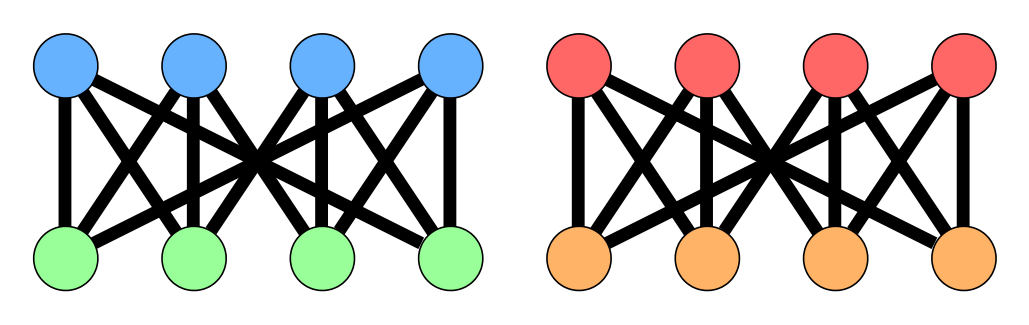
\includegraphics[width=\textwidth]{images/graph_1}
			\caption{Граф 1}
			\label{fig:graph1}
		\end{minipage}
		\hfill
		\begin{minipage}[b]{0.4\textwidth}
			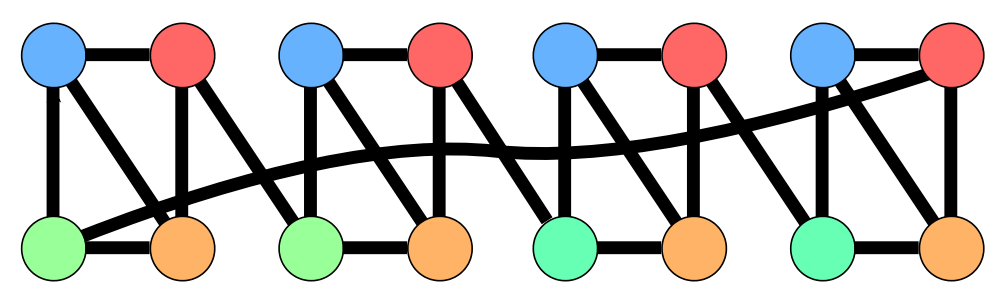
\includegraphics[width=\textwidth]{images/graph_2}
			\caption{Граф 2}
			\label{fig:graph2}
		\end{minipage}
	\hfill
	\end{figure}
	
	
	Возьмем произвольное ребро $ (\xi, \eta) \in E $. Тогда классы вершин, соединяемых этим ребром, $y_{\xi}$ и $y_{\eta} $ соответственно.
	Задача метрики состоит в том, чтобы показать, сколько информации о классе $ y_{\eta} $ дает знание $ y_{\xi} $.
	Энтропия $ H(y_{\xi}) $ измеряет «трудность» предсказания метки $ \xi $ без знания $ y_{\eta} $.
	При заданном $ y_{\eta} $ это значение сводится к условной энтропии $ H(y_{\xi}|y_{\eta}) $.
	Другими словами, $ y_{\eta} $ раскрывает $ I(y_{\xi},y_{eta}) = H(y_{\xi}) − H(y_{\xi}|y_{\eta}) $ информации о метке.
	Из этого можно посчитать label informativeness для отдельного класса:
	
	$$ LI := \frac{I( y_{\xi}, y_{\eta} )}{H(y_{\xi})} $$
	
	Полученная метрика LI принадлежит интервалу [0, 1], при $ LI = 1 $ знание класса $ y_{\xi} $ позволяет однозначно узнать класс $ y_{\eta} $, а при $ LI = 0 $ метки классов не зависят друг от друга.
	При этом, метрика в зависимости от выбранного распределения может принимать различный вид. Например, если ребра выбираются из равномерного распределения, мы получаем формулу:
	
	$$ LI_{edge} = - \frac{ \sum_{c_1, c_2} p(c_1, c_2) log \frac{ p(c_1, c_2) }{ \bar{p}(c_1) \bar{p}(c_2) } }{ \sum_c \bar{p}(c) log \bar{p}(c) } = 2 - \frac{  \sum_{c_1, c_2} p(c_1, c_2)  log p(c_1, c_2) }{ \sum_c \bar{p}(c) log \bar{p}(c) } $$
	где $$ p(c_1, c_2) = \sum_{u, v \in E} \frac{ [y_u = c_1, y_v = c_2] }{ 2|E| } $$
	
	Полученная метрика:
	\begin{itemize}
		\item Удовлетворяет maximal agreement, так как принимает значение 1 в случае, когда знание класс одного из конец ребра позволяет однозначно определить класс второго.
		
		\item Удовлетворяет constant baseline через еще одно объемное доказательство. (Это доказательство достаточно громоздкое, лежит в appendix С работы).
	\end{itemize}
	
	\subsection{Генерация синтетических данных}
	
	Для того, чтобы контролировать характеристики создаваемого графа предлагается использовать стохастическую блочную модель (SBM) \cite{holland1983stochastic}.
	Вершины в этой модели разделены на C классов.
	Любую пару вершин $i,j$ можно соединить ребром с вероятностью $p_{c(i)c(j)}$  независимо от других вершин.
	Здесь $c(i)$ соответствует классу вершины $i$ или искомой метке вершины.
	
	Возьмем  количество классов равное $C=4$, размеры классов одинаковые $l=n/4$, тогда вероятность соединения вершин $p_{i,j}$ можно записать следующим образом:
	
	$$p_{i,j} = \begin{cases}
		p_0K, & \text{если } i = j,\\
		p_1K, & \text{если } i + j = 5,\\
		p_2K, & \text{в остальных случаях},\\
	\end{cases}$$
	
	где $p_0+p_1+2p_2=1$ и $K$ положительное число.
	При этом среднее ожидаемая степень любой вершины будет равна $p_0 Kl+p_1 Kl+2p_2 Kl=Kl$.
	
	Данная модель позволяет получить граф с различными характеристиками.
	Коэффициент $p_0$ позволяет контролировать уровень гомофилии в графе, а соотношение между $p_1$ и $p_2$ позволяет влиять на LI графа.
	
	Манипуляцию характеристиками графа можно объяснить следующим образом: есть соотношение $i+j=5$, по нему ребрами соединяются пары вершин с классами (1, 4) и (2, 3).
	Тогда при $p_2=0$ и $p_1>0$, зная метки классов соседей можно точно предсказать метку текущей вершины.
	Если же есть отношение $p_1=p_2$, то сложно дать какую-либо точную информацию о метке текущей точки.
	Во время манипуляций с $p_1$ и $p_2$  на $p_0$ не накладывались дополнительные ограничения, хотя именно эта величина характеризует уровень гомофилии в создаваемом графе.
	
	Для того, чтобы определить границы характеристик, которые могут быть получены при помощи данной модели необходимо вычислить асимптотические значения.
	
	При $n \rightarrow \infty$:
	
	$$h_{adj} = \dfrac{4}{3}p_0 - \dfrac{1}{3}$$
	
	$$LI = 1 - \dfrac{H(p_0,p_1,p_2,p_2)}{\log 4}$$
	
	где $H(X) = -\sum_ix_i\log(x_i)$
	
	Получается, $h_adj$ может принимать значения от $-1/3$ до $1$, $LI$ может быть от $0$ до $1$. Если $LI=0$, тогда всегда $h_{adj}=0$; если $h_{adj}=1$ то и $LI=1$.
	Но если $LI=1$, то $h_{adj}=1$ или $h_{adj}=-1/3$.
	
	\pagebreak
	\section{Описание данных для экспериментов, результаты применения на данных, потенциал и области прикладного применения методов}
	\setcounter{figure}{0}
	
	В данном разделе исследуется взаимосвязь между характеристиками графа и качеством GNN.
	В предыдущих исследованиях было показано, что GNN способны показывать хорошее качество на не гомофильных наборах данных.
	Предполагается, что GNN могут выделять из графов более сложные отношения, чем просто гомофилию.
	При этом ожидается, что GNN будет работать до тех пор, пока окружение вершины содержит некоторую информацию о ней.
	Предлагается использовать LI для измерения информативности окружения вершин графа.
	
	Для проверки данной гипотезы были собраны различные наборы реальных данных, а также получен способ для генерации графов на основе стохастической блочной модели с предсказуемыми коэффициентами гомофилии и LI.
	
	Для генерации графов был составлено 208 различных комбинаций $p_0,p_1,p_2$ для получения различных характеристик LI и гомофилии.
	Для каждой комбинации генерировалось 10 графов, в каждом из которых по 1000 вершин со степенью 10.
	Признаки вершин брались из набора данных cora \cite{mccallum2000automating},\cite{namata2012query},\cite{sen2008collective} и \cite{yang2016revisiting}.
	Полученные графы делились на обучающую/валидационную/тестовую выборки в соотношении 50\%/25\%/25\%.
	
	В качестве GNN моделей использовались GCN \cite{kipf2016semi} и GraphSAGE \cite{hamilton2017inductive}.
	
	\subsection{Результаты работы с синтетическим наборами данных на основе стохастической блочной модели}

	На графиках (см. рисунки \ref{fig:accuracy-of-graphsage} и \ref{fig:accuracy-of-gcn}) представлено качество обученных GNN сетей.
	Каждая точка соответствует сгенерированному набору данных, при этом по оси X откладывается метрика $h_adj$, по оси Y LI, цвет отражает Accuracy полученной модели. 
	
	Разберем график с изображением качества модели GraphSAGE (см. рисунок \ref{fig:accuracy-of-graphsage}).
	По нему видно, что качество модели больше коррелирует с LI, чем с гомофилией.
	Действительно, коэффициент корреляции Спирмена между accuracy и LI равен 0.93, а между accuracy и гомофилией 0.05.
	Если показатель LI высокий, то accuracy GraphSAGE остается также высоким несмотря на отрицательный коэффициент гомофилии.
	Для модели GCN наблюдается аналогичная ситуация (см. рисунок \ref{fig:accuracy-of-gcn}).

	\begin{figure}[!tbp]
		\centering
		\begin{minipage}[b]{0.4\textwidth}
			\includegraphics[width=\textwidth]{"images/Accuracy of GraphSAGE"}
			\caption{Accuracy GraphSAGE модели на синтетических графах}
			\label{fig:accuracy-of-graphsage}
		\end{minipage}
		\hfill
		\begin{minipage}[b]{0.4\textwidth}
			\includegraphics[width=\textwidth]{"images/Accuracy of GCN"}
			\caption{Accuracy GCN модели на синтетических графах}
			\label{fig:accuracy-of-gcn}
		\end{minipage}
	\end{figure}

	\subsection{Полусинтетические данные из \cite{ma2021homophily}}
	
	В \cite{ma2021homophily} авторы выявили, что GNN показывает хорошие результаты на некоторых гетерофильных наборах данных.
	Были получены полусинтетические графы при помощи добавления межклассовых ребер согласно паттернам из реальных графов.
	Это позволило получить набор данных с графами с разными уровнями гомофилии.
	
	Для выявления причины выявленного изменения качества была обучена GraphSAGE модель на полусинтетических данных (как в \cite{ma2021homophily}) основанных на cora графе.
	Было выявлено, что модель получает хорошее качество, когда граф имеет высокий уровень LI.
	Зависимость между LI, $h_{adj}$ и accuracy показана на рисунке 4. 
	Коэффициент корреляции Спирмена между accuracy и LI равен 0.78, а между accuracy и гомофилией -0.24. 
	
	
	Аналогичный опыт был проведен для графа citeseer, график результатами приведен на рисунке \ref{fig:accuracy-of-graphsage-citeseer}.
	Коэффициент корреляции Спирмена между accuracy и LI равен 0.51, а между accuracy и гомофилией -0.54.
	
	\begin{figure}[H]
		\centering
		\begin{minipage}[b]{0.4\textwidth}
			\includegraphics[width=\textwidth]{"images/Accuracy of GraphSAGE cora"}
			\caption{Accuracy GraphSAGE модели на полусинтетическом cora наборе данных \cite{ma2021homophily}}
			\label{fig:accuracy-of-graphsage-cora}
		\end{minipage}
		\hfill
		\begin{minipage}[b]{0.4\textwidth}
			\includegraphics[width=\textwidth]{"images/Accuracy of GraphSAGE citeseer"}
			\caption{Accuracy GraphSAGE модели на полусинтетическом citeseer наборе данных \cite{ma2021homophily}}
			\label{fig:accuracy-of-graphsage-citeseer}
		\end{minipage}
	\end{figure}
	

	
	\subsection{Синтетические данные из \cite{luan2021heterophily}}
	
	В  статье \cite{luan2021heterophily} авторы также приходят к выводу, что GNN показывает хорошее качество на некоторых гетерофильных графах.
	Авторы исследовали зависимость качества GNN сетей на различных уровнях гомофилии.
	Было выявлено, что график этой зависимости имеет U форму, т.е. наблюдается высокое качество GNN модели как при высоких значениях гомофилии, так и при низких.
	
	Были сгенерированы данные аналогично \cite{luan2021heterophily}. Для каждого полученного графа был рассчитан уровень LI (см. рисунок \ref{fig:label-informativeness-depending-on-edge-homophily}).
	График зависимости LI от edge homophily также имеет U форму.
	Отсюда можно сделать вывод, что GNN модели из \cite{luan2021heterophily} хорошо работают при высоких значениях LI.
	
	\begin{figure}[H]
		\centering
		\includegraphics[width=0.4\linewidth]{"images/Label informativeness depending on edge homophily"}
		\caption{LI в зависимости от $h_{edge}$ на синтетическом графе \cite{luan2021heterophily}}
		\label{fig:label-informativeness-depending-on-edge-homophily}
	\end{figure}
	
	
	\pagebreak
	
	\section*{ \hfill ЗАКЛЮЧЕНИЕ \hfill}
	\addcontentsline{toc}{section}{\protect\numberline{}ЗАКЛЮЧЕНИЕ}
	
	В результате выполнения работы были получены следующие основные результаты и выводы.
	
	
	
    \pagebreak
    \renewcommand{\refname}{{ \hfill СПИСОК ИСПОЛЬЗОВАННЫХ ИСТОЧНИКОВ \hfill}}
    \addcontentsline{toc}{section}{\protect\numberline{}СПИСОК ИСПОЛЬЗОВАННЫХ ИСТОЧНИКОВ}
%    \bibliographystyle{unsrt}
    \selectbiblanguage{russian}
    \bibliographystyle{BibTeX-Styles/ugost2008mod}
    \bibliography{main}
    \newpage

\end{document}